\section{Conclusion} \label{conclusion}
In the formulation of the research questions we already mentioned that there is not a single structure that can do it all. There is always a mix of trade-offs. So one thing we can do is optimize the parts that are the same for the desired structures and then build specialized structures around that. This method is described in Section \ref{approach:flipbook_animations}. During this thesis, a VDB structure was implemented as it was a balance between structure size, sample timing and efficient HDDA. This structure along with our voxel data compression scheme allowed us to load in full animation sequences into our engine and render them at movie-level fidelity. Compared to previous techniques \cite{dolonius2017compressing}, that compresses RGB data to between $26.7$ and $10.7$ bits per voxel (between $7$ and $17$ times reduction over their original data), we have a better bits per voxel ratio, but do not achieve the same compression rates compared to our original data due to f16 voxels already being smaller than 24-byte RGB color values. Our block compression scheme allows for an $8\times$ reduction in memory usage over the standard 16-bit floating point format. Along with that, we can get another reduction by between $14\%$ and $57\%$ without significant quality loss by clustering voxel bricks which contain roughly the same data. Both of these compression methods do not work for all models out of the box, some models might need to be slightly altered to prevent edge cases as seen in \ref{fig:block_compression:fire_unorm}. In Table \ref{tab:tracing_performance:numbers} we see that our main bottleneck when rendering volumes using a sampling technique is computation (ALU bound), instead of memory. The same problem arises with our HDDA implementation, which has low occupancy due to high register usage, but this is not an issue as long as we are not memory-bound. Both of these results are surprising as GPU algorithms are most often memory-bound due to the large number of pixels and buffers that have to be read and written to. So when optimizing the implemented methods the main point of interest would be to reduce the number of steps taken and reduce the register usage of our HDDA implementation. The former can likely be achieved by utilizing a signed distance field as described in Section \ref{related_work:attribute_separation:fast_volume_traversal}. A summary of this conclusion is written below by covering each of the listed requirements (as mentioned in Chapter \ref{requirements}):

\begin{enumerate}
    \item The \textbf{Asset size} issues of volume data structures are partially solved. Our voxel data has been compressed to the point where most models use less than 64 MB. And by far our largest model (in terms of number of voxels), Shockwave, uses 256 MB for its voxel data. Unfortunately our tree sizes have not been optimized for animations yet which results in each animation frame linearly increasing the tree size by 20 to 30 MB, making long animation sequences impractical.
    \item The \textbf{Sampling speed} is fast enough to utilize real time frame rates when using a technique like delta tracking as described in Section \ref{related_work:path_traced_volume_rendering:delta_tracking}, or ray marching as shown in Figure \ref{fig:tracing_performance:fog_volume}. HDDA traversal, as described in Section \ref{related_work:attribute_separation:fast_volume_traversal} is also fast enough to run in real time.
    \item \textbf{Animation playback} is practically free as we only have to change the starting position of our tree traversal which is done by changing the animation frame index.
    \item \textbf{Lossy compression} is effective to the point of reducing our voxel data by between 9 to 18 times, by utilizing both compression techniques, without significantly losing visible quality in most cases.
    \item \textbf{Level of detail} could be added by mip-mapping one level of the voxel data texture. Additional data per internal node could also be added. No testing or benchmarking for either of these techniques has been done though.
\end{enumerate}


\subsection{Renders}
\begin{figure}[H]
    \centering
    \subfloat[Path traced half resolution Disney Cloud path traced using multiple scattering.]{
        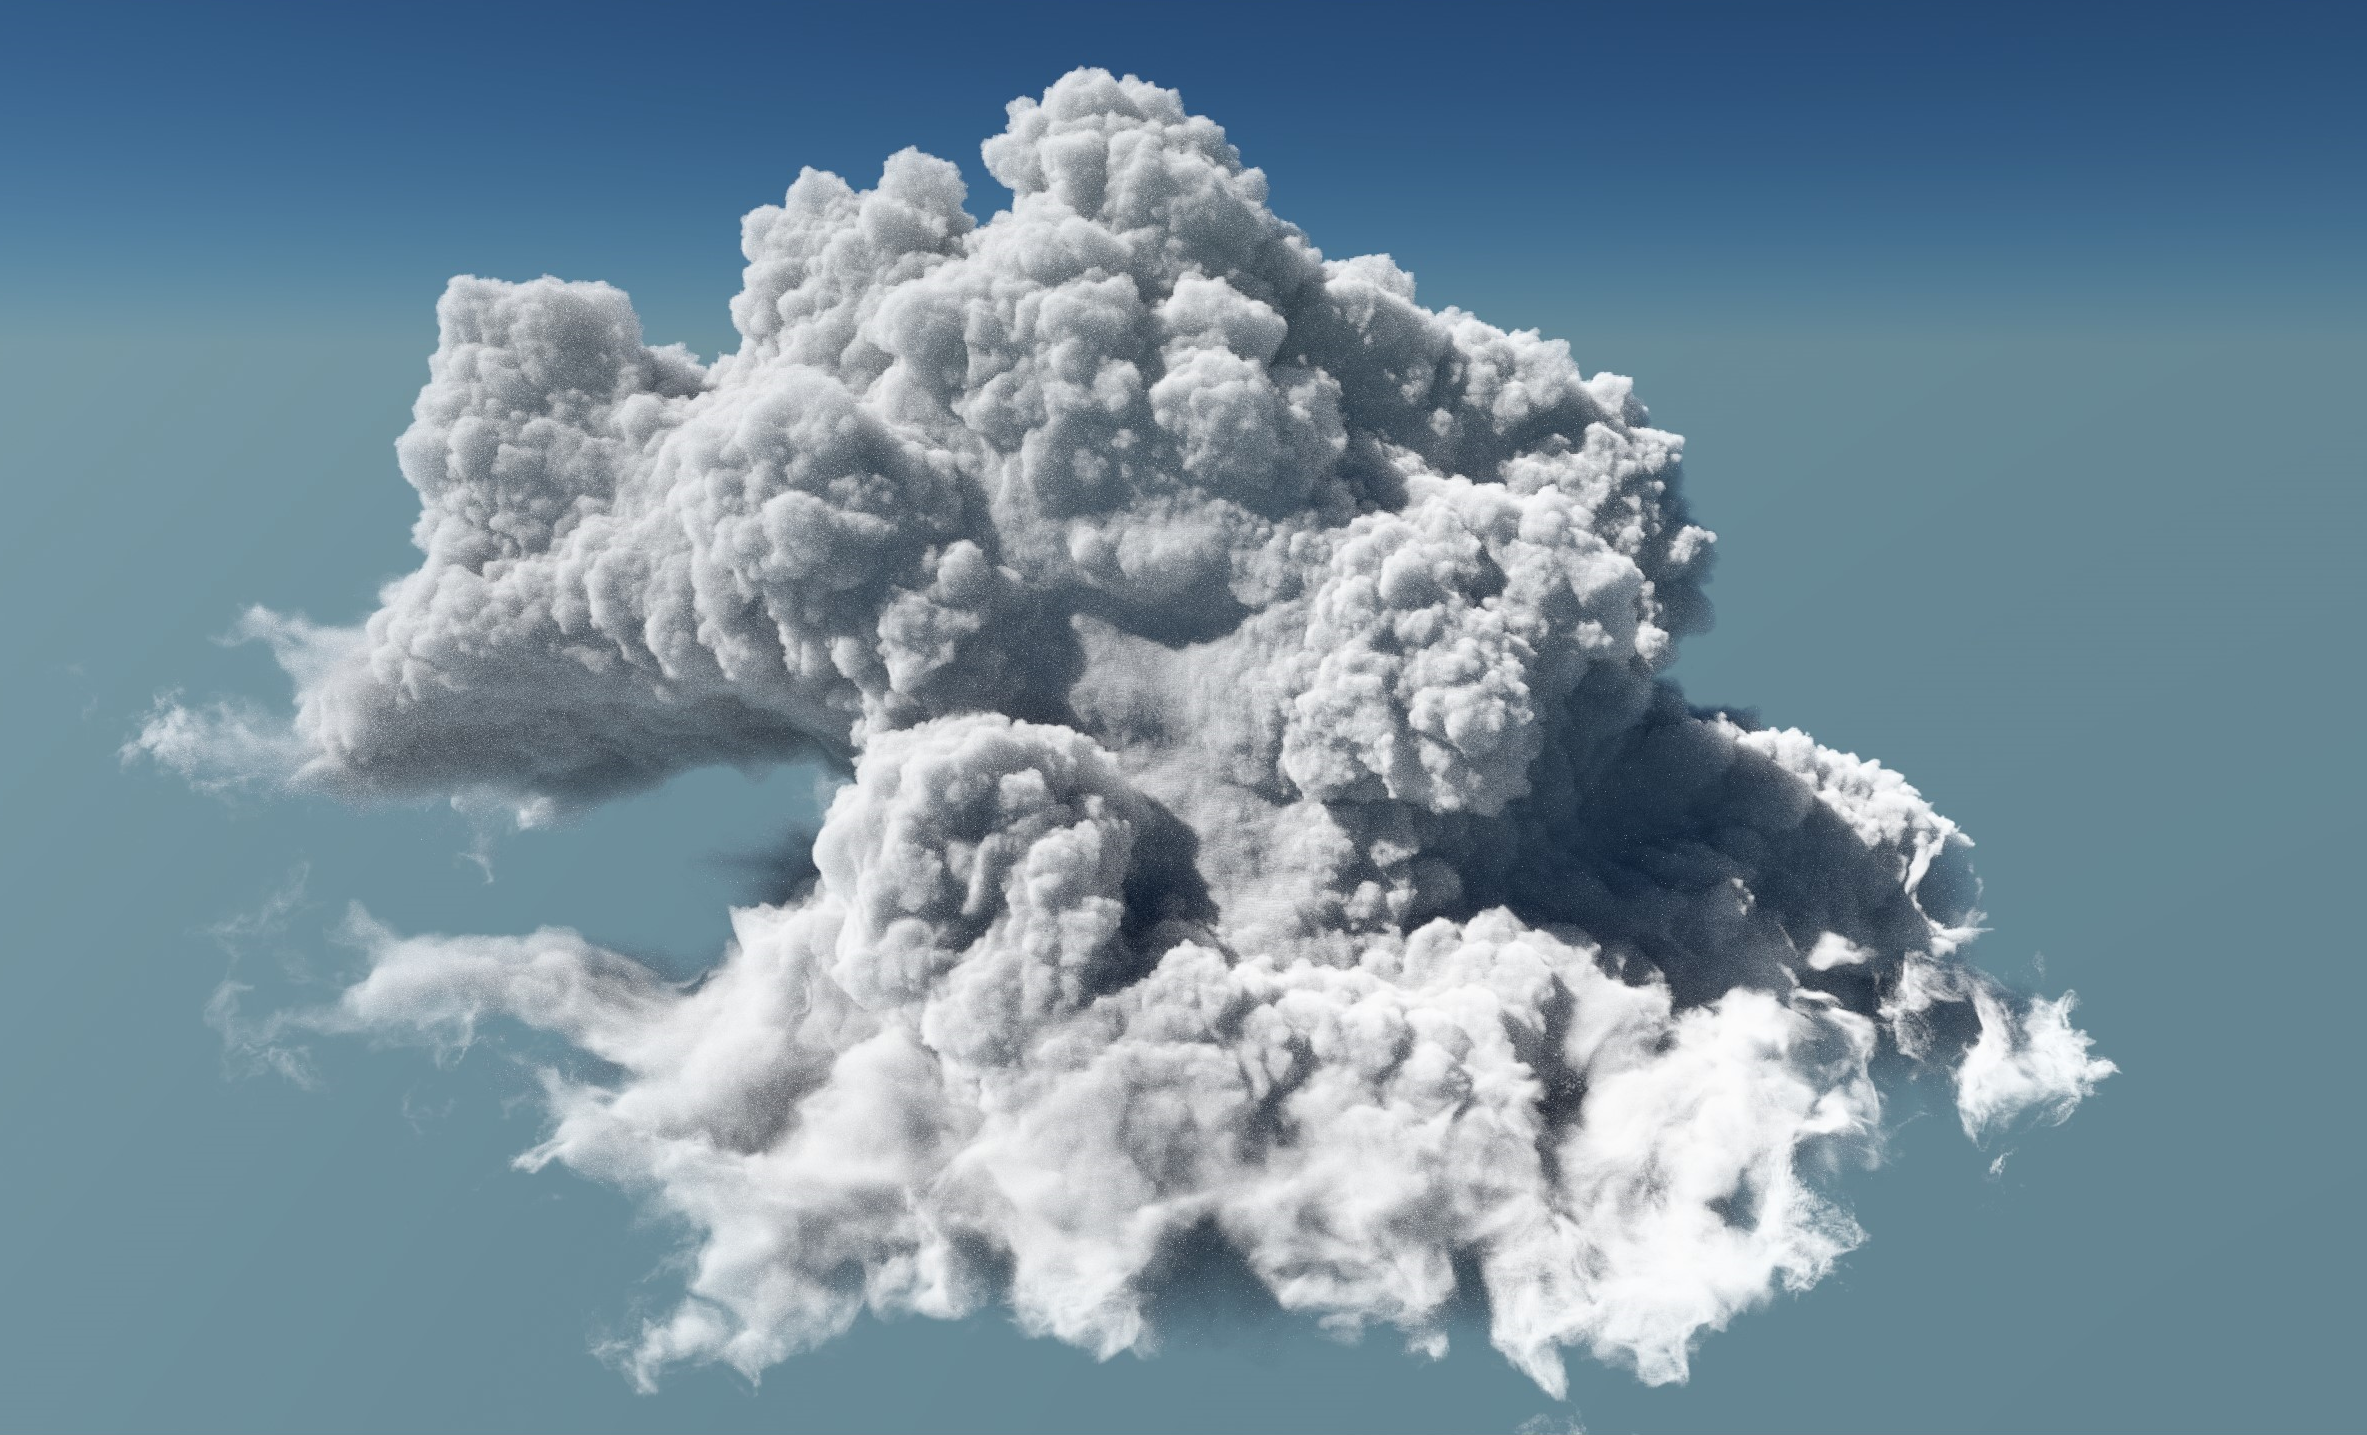
\includegraphics[width=0.9\textwidth]{figures/disney _cloud.png} \label{fig:renders:disney_cloud}
    }
    \hfill
    \subfloat[Ray marched smoke inside the Bistro scene coming from a chimney.]{
        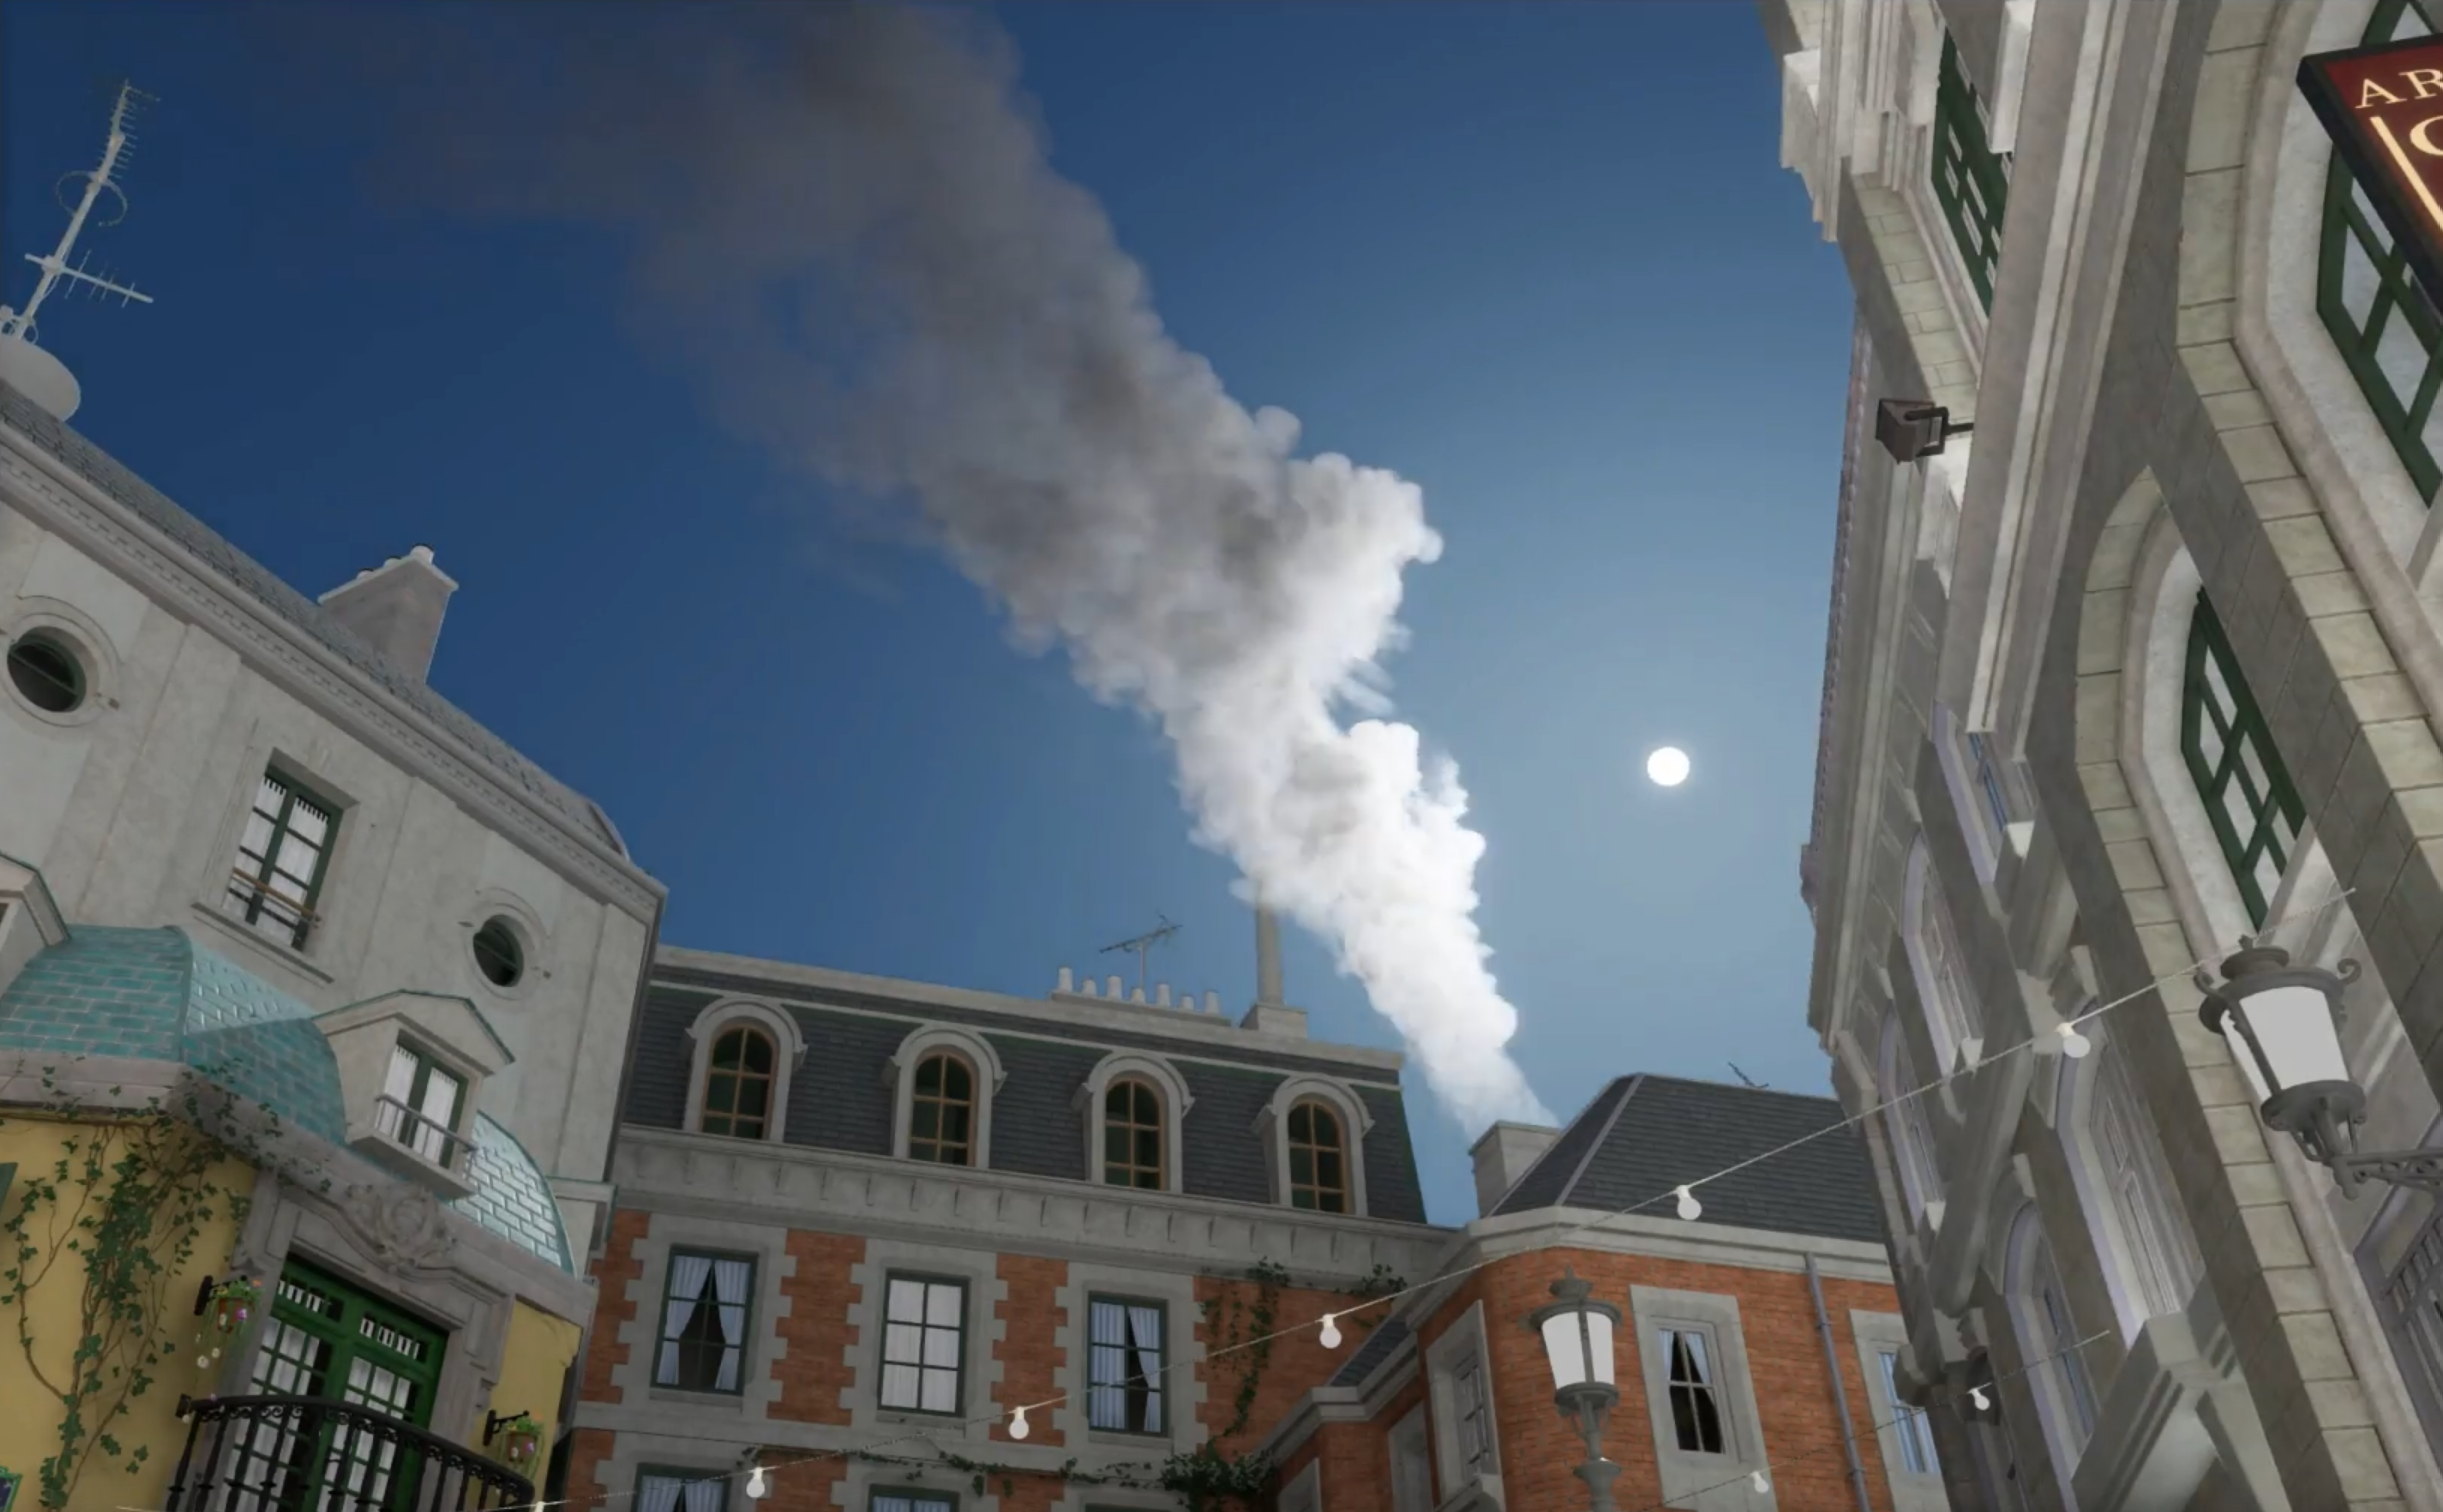
\includegraphics[width=0.45\textwidth]{figures/bistro_chimney_0.png} \label{fig:renders:bistro_0}
    }
    \hfill
    \subfloat[The same scene later on the day shows a different frame in the animation sequence.]{
        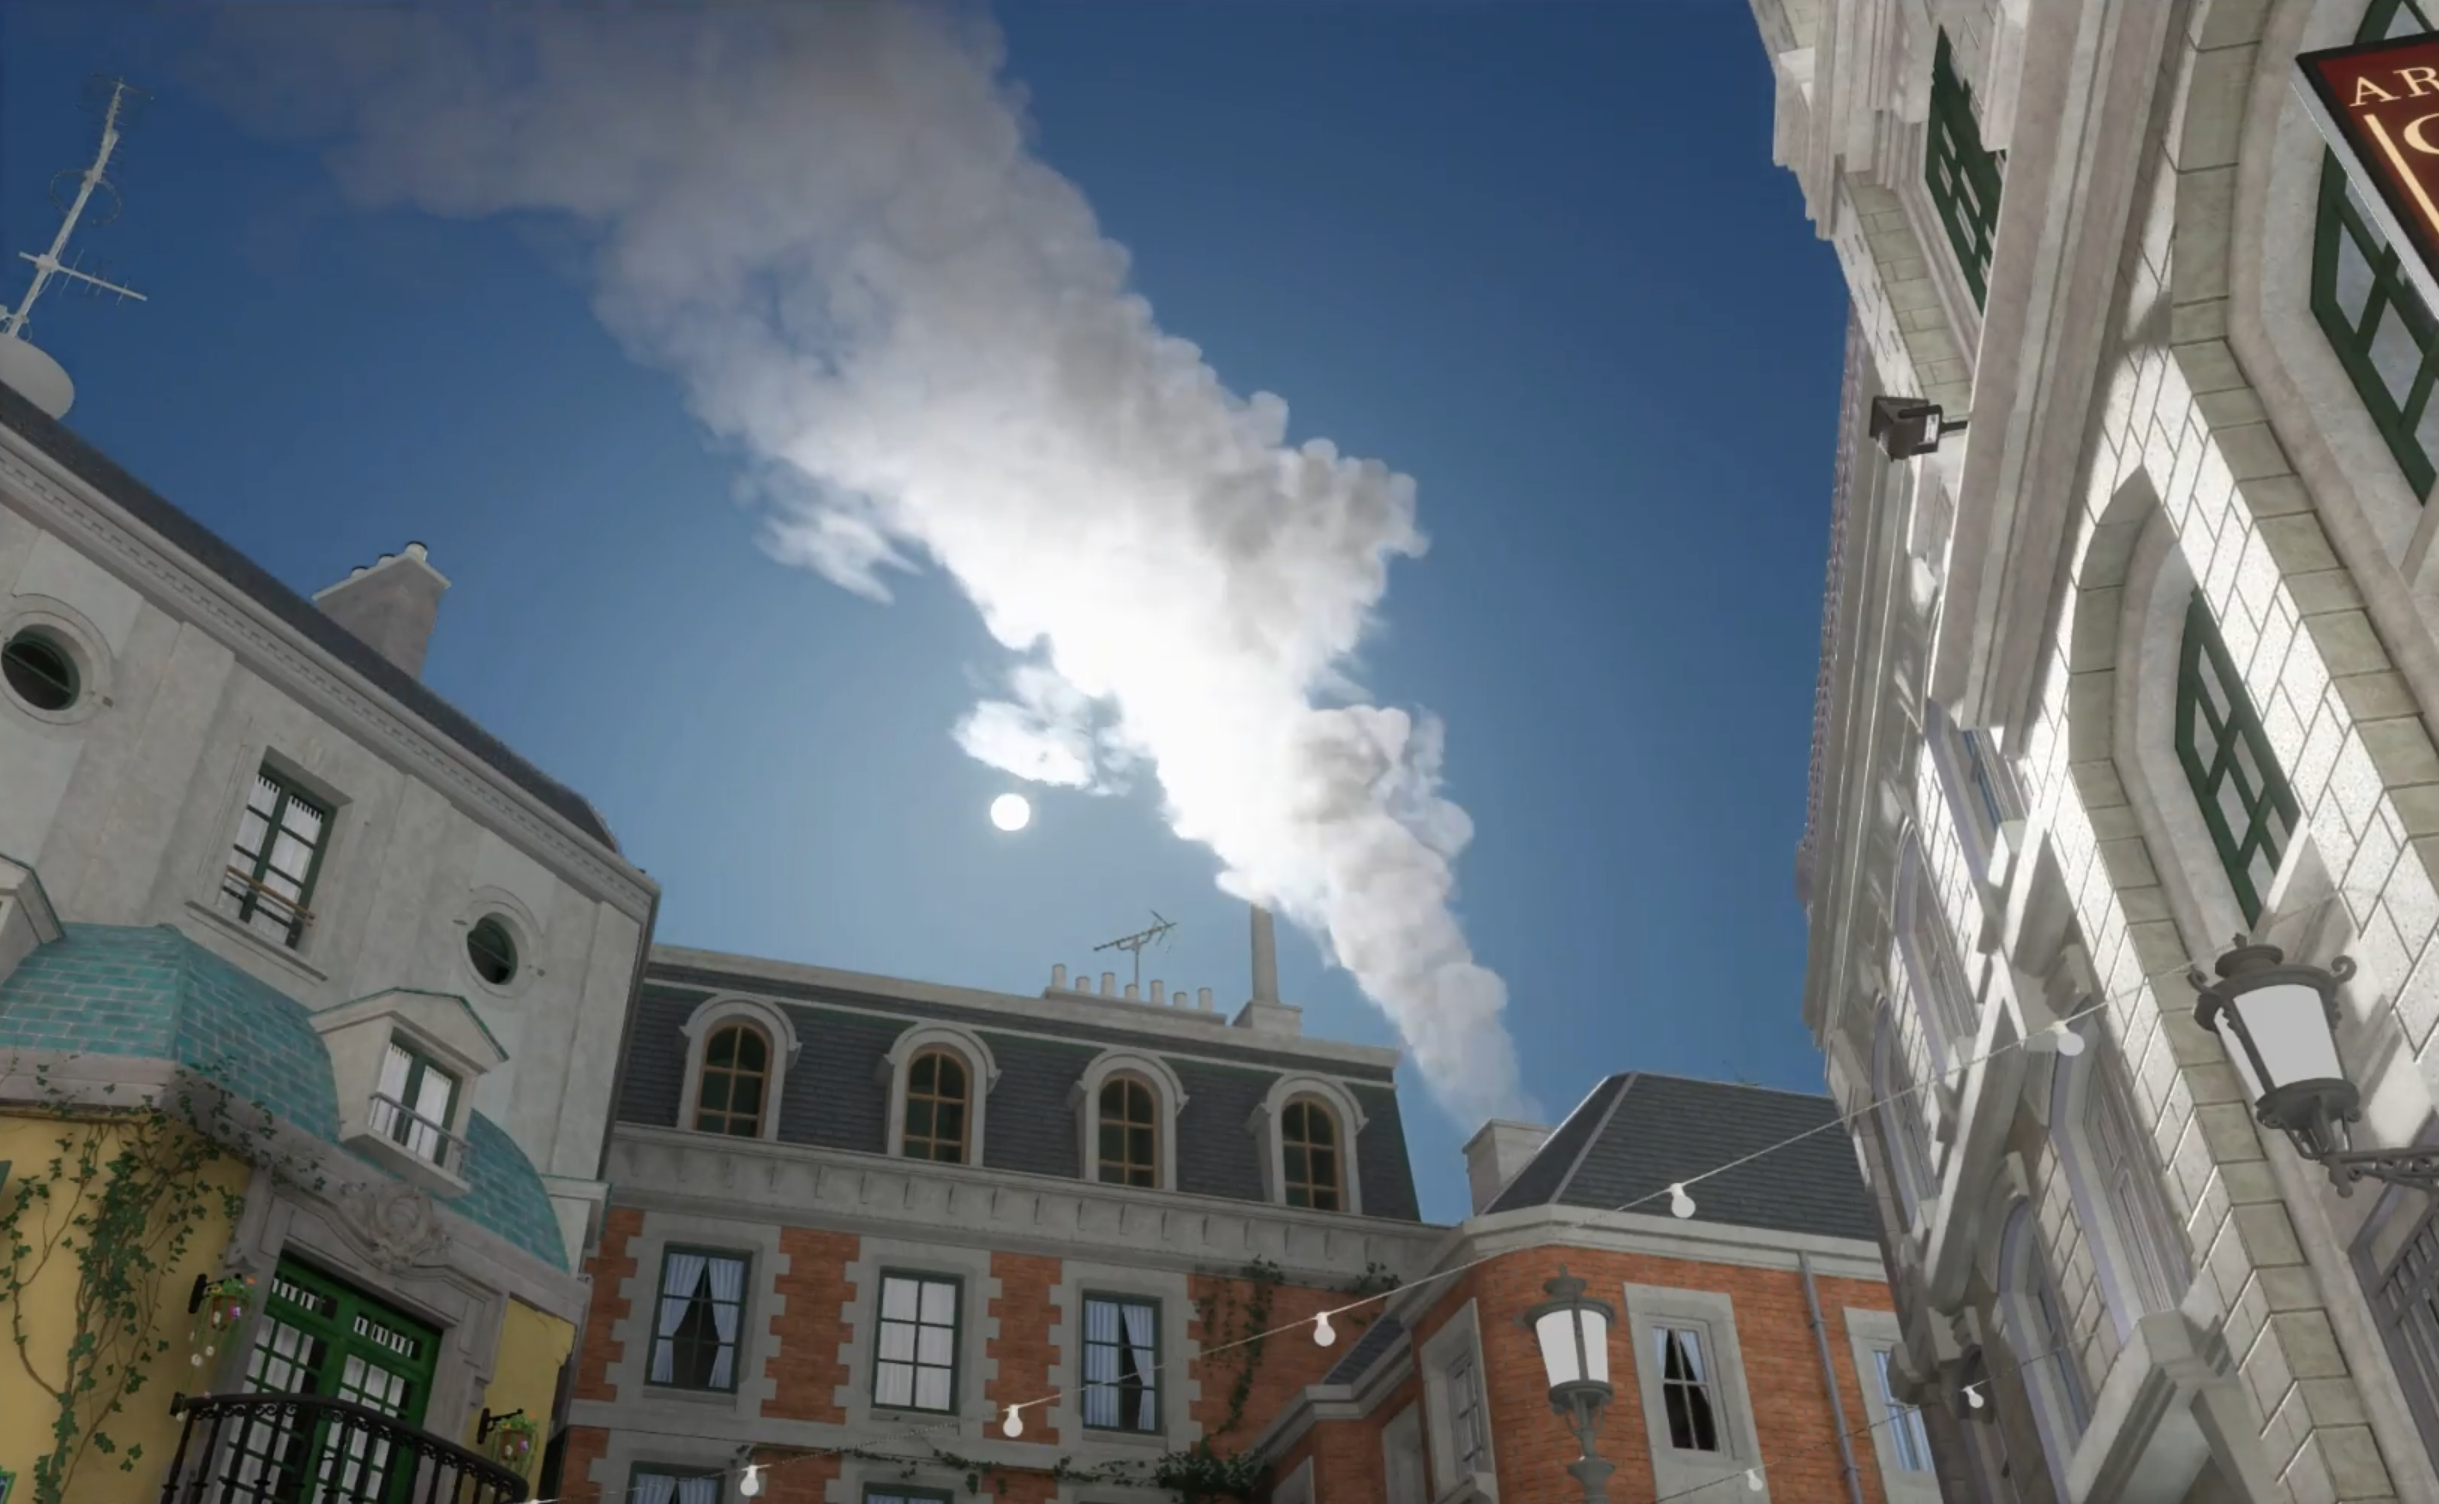
\includegraphics[width=0.45\textwidth]{figures/bistro_chimney_1.png} \label{fig:renders:bistro_1}
    }

    \hfill

    \caption{Multiple renders made in Breda using the created data structures. Figure \ref{fig:renders:disney_cloud} shows the largest tested model which was rendered by using path tracing. This was not real-time (about 5 frames per second) because we use multiple scattering, which means that our ray can bounce many times into different directions within the cloud. Figures \ref{fig:renders:bistro_0} and \ref{fig:renders:bistro_1} show two frames from a video made in the Bistro scene. This was rendered using our ray marcher which does run in real-time together with all other systems in Breda. The way that the light dynamically scatters throughout the chimney smoke is an effect that is currently not done in any AAA game.} \label{fig:renders}
\end{figure}

\newpage
\subsection{Future research} \label{conclusion:future_research}

\begin{itemize}
    \item One point of improvement to the in Section \ref{approach:clustering_similar_nodes} mentioned clustering method could be a more optimized rejection scheme. Currently, we reject if the normalized variance of all brick values is too high. This only allows us to cluster homogeneous bricks and not bricks that contain a smooth gradient, even though there are bricks that are simply a gradient in one specific axis which likely could be clustered. In the future, different distance functions could be used. This could reduce the dependance on our rejection scheme, and maybe purely rely on clustering. 
    \item Another major issue with the clustering compression scheme are the build times. It currently takes multiple minutes to compress both the shockwave and the chimney animation, which makes development iteration times very slow.
    \item Different texture compression schemes can be experimented with. Certain platforms, like mobile, have different texture compression formats namely, Ericsson Texture Compression (ETC) and Adaptive scalable compression (ASTC). ETC has 1 bit per voxel which is twice the compression ratio of the method described in \ref{approach:texture_compression}. And ASTC can compress between $0.15$ and $1.19$ depending on certain options. These compression schemes will change the quality of our data but might be worth it on the supported platforms.
    \item Different tree topologies can be experimented with. Most notably B+Tree's with uniform layer sizes (unlike our current setup with node sizes $32^3$, $16^3$ and $8^3$). This might make it possible to deduplicate many of the bit masks and thus shrink the tree size. Another benefit as mentioned in \cite{hoetzlein2016gvdb}, by using a tree where all internal nodes are $8^3$ we get better ray tracing performance.
    \item The ideas about running simulations inside our VDB data structure as described in Section \ref{approach:simulation} can be implemented. During this research, there was a very limited time investment in making this feature work. So experimenting with the theorized technique could result in a nice piece of follow-up research.
\end{itemize}

